\documentclass[12pt]{article}

\usepackage{fixltx2e}
\usepackage{textcomp}
\usepackage{fullpage}
\usepackage{amsfonts}
\usepackage{verbatim}
\usepackage[english]{babel}
\usepackage{pifont}
\usepackage{color}
\usepackage{setspace}
\usepackage{lscape}
\usepackage{indentfirst}
\usepackage[normalem]{ulem}
\usepackage{booktabs}
% \usepackage{nag}
\usepackage{natbib}
% \usepackage{bibtex}
\usepackage{float}
\usepackage{latexsym}
\usepackage{hyperref}
\usepackage{url}
% \usepackage{html}
\usepackage{epsfig}
\usepackage{graphicx}
\usepackage{amssymb}
\usepackage{amsmath}
\usepackage{bm}
\usepackage{array}
%\usepackage{mhchem}
\usepackage{ifthen}
\usepackage{caption}
\usepackage{xcolor}
\usepackage{amsthm}
\usepackage{amstext}
\usepackage{nicefrac}
\usepackage{algorithm}
\usepackage{algorithmic}
\usepackage[scientific-notation=true]{siunitx}
\usepackage{subfigure}
\usepackage[flushleft]{threeparttable}
\usepackage{lineno}
\usepackage{adjustbox}

\begin{document}

\begin{minipage}[h]{\textwidth}
	\title{StarBEAST2 enables accurate and precise inference of species trees, divergence times and clock rates}
	\author{Huw A. Ogilvie$^{\ast,1,2}$ and Alexei J. Drummond,$^{2,3}$}
    \maketitle
\end{minipage}

\raggedright
$^{1}$Department of Evolution, Ecology and Genetics, Australian National University, Canberra, Australia\\
$^{2}$Centre for Computational Evolution, University of Auckland, Auckland, New Zealand\\
$^{3}$Department of Computer Science, University of Auckland, Auckland, New Zealand

\clearpage

\section{Abstract}

Keywords: Phylogenetic methods, substitution rate, relaxed clock, multispecies coalescent, concatenation.

\section{Introduction}


\section{New Approaches}


\section{Results}

\clearpage

\begin{figure}[htb!]
\centering
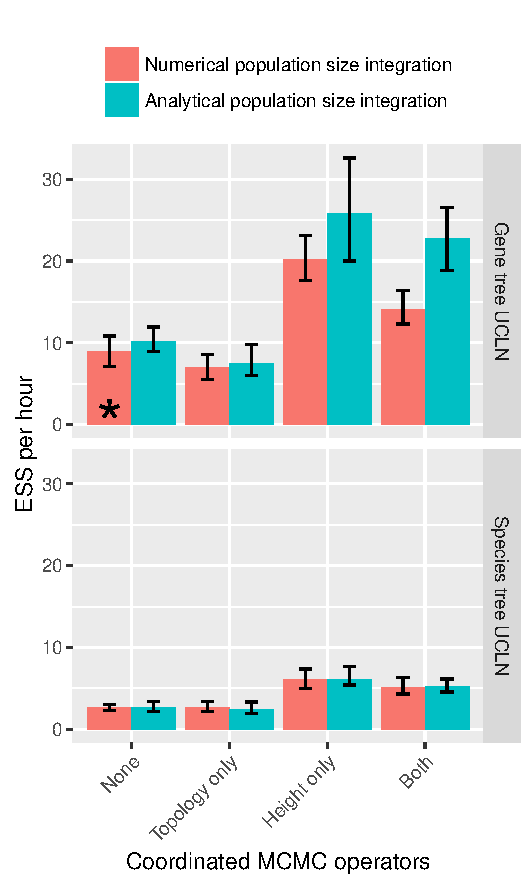
\includegraphics[height=14cm]{speciesTreeHeight_ess_per_hour.pdf}
\caption
{Mean estimated sample size (ESS) per hour of the \textit{Pseudacris} species tree height.}
\label{fig:essPerHour}
\end{figure}

\clearpage

\begin{figure}[htb!]
\centering
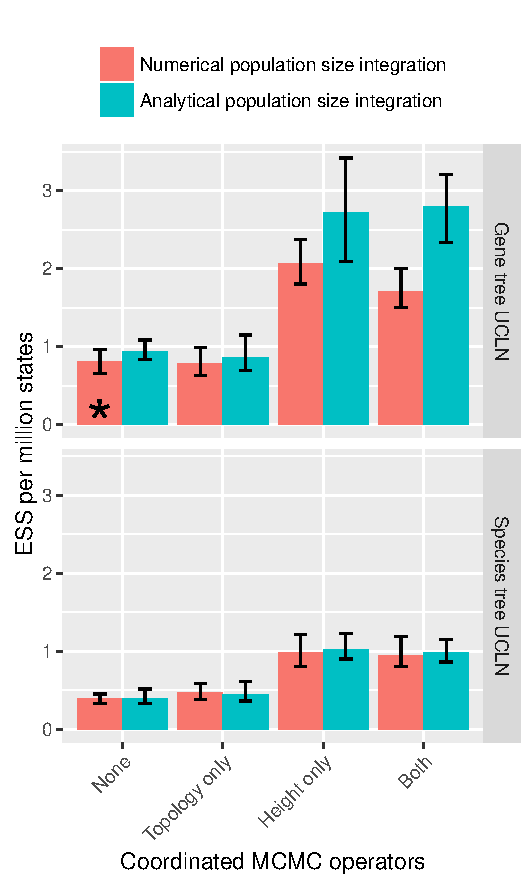
\includegraphics[height=14cm]{speciesTreeHeight_ess_per_mstates.pdf}
\caption
{Mean estimated sample size (ESS) per million states of the \textit{Pseudacris} species tree height.}
\label{fig:essPerMstates}
\end{figure}

\clearpage

\begin{figure}[htb!]
\centering
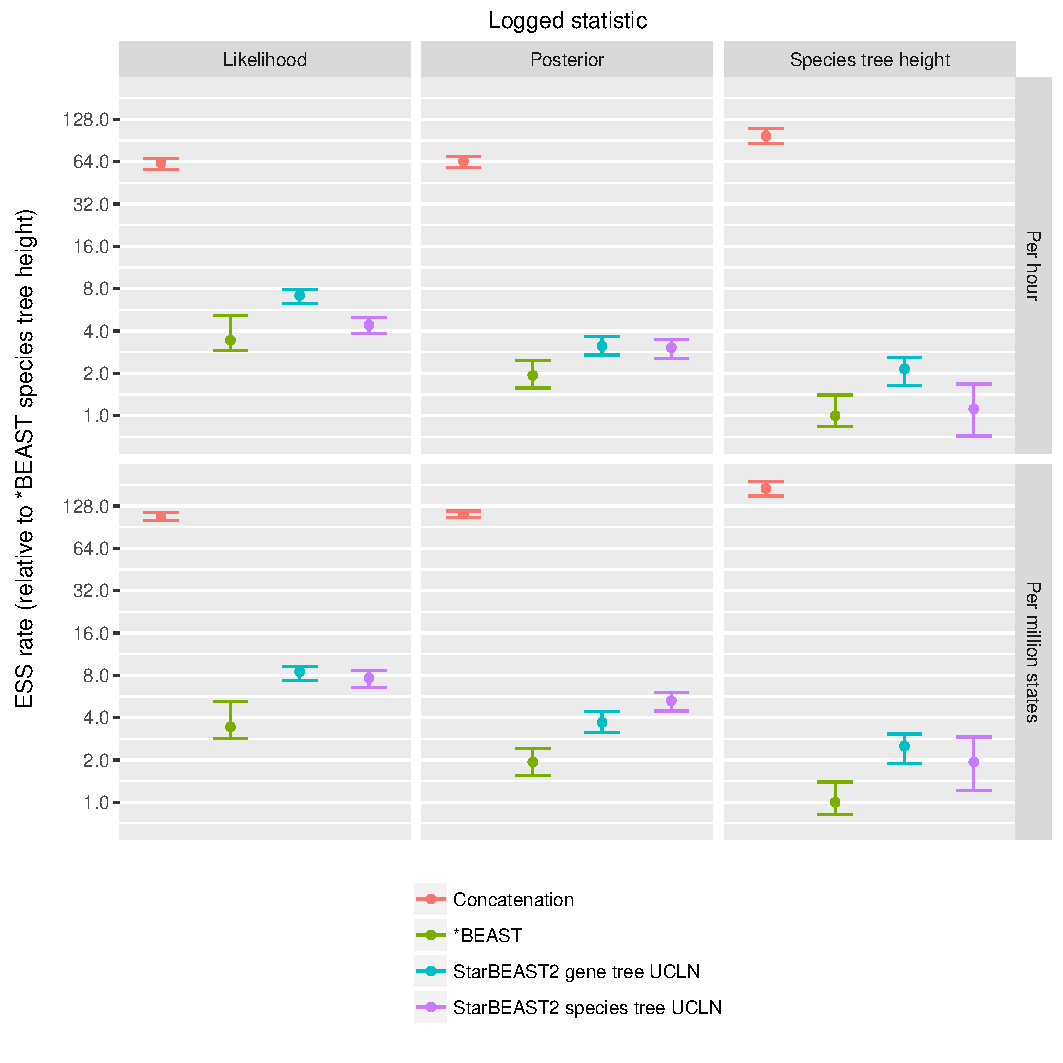
\includegraphics[height=17cm]{multiple.pdf}
\caption
{Comparison of estimated sample size (ESS) rates using different methods applied to simulated alignments.}
\label{fig:loggedStatistics}
\end{figure}

\clearpage

\begin{figure}[htb!]
\centering
\includegraphics[height=9cm]{species_tree_error.pdf}
\caption
{Comparison of the accuracy of different methods applied to simulated alignments.}
\label{fig:speciesTreeError}
\end{figure}

\clearpage

\begin{figure}[htb!]
\centering
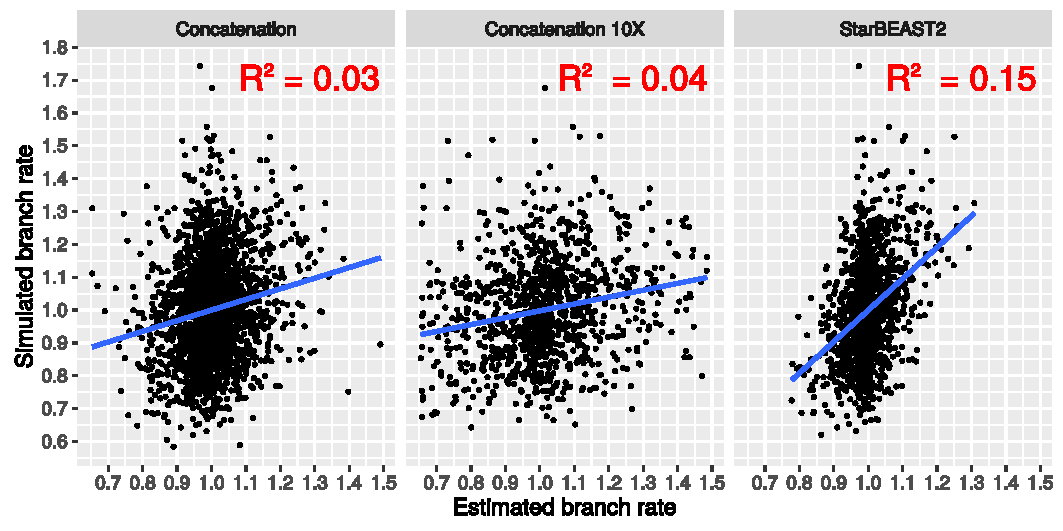
\includegraphics[height=14cm]{branch_rates_lm.pdf}
\caption
{Recovery of species tree branch rates using concatenation and StarBEAST2.}
\label{fig:branchRatesLM}
\end{figure}

\clearpage

\section{Discussion}


\section{Materials and Methods}


\section{Supplementary Material}
Supplementary tables XX-XX and figures XX-XX are available at \textit{Molecular Biology and Evolution} online (http://www.mbe.oxfordjournals.org/).


\section{Acknowledgments}
Blah blah blah


\bibliographystyle{natbib}
\bibliography{starbeast2}

\end{document}
